\documentclass[slidetop,11pt]{beamer}
%
% Packages pour le francais
\usepackage[T1]{fontenc}
\usepackage[latin1]{inputenc}
\usepackage[frenchb]{babel}

%
% pour un pdf lisible a l’ecran
% il y a d’autres choix possibles
\usepackage{pslatex}
%
% pour le style et couleurs
\usetheme{Boadilla}
%
% contenu de la page de titre
\title{When is a Periodic Function the Curvature of a Closed Plane Curve?}
\subtitle{From an article of J. Arroyo, O. J. Garay and J. J. Mencia}
\date{\oldstylenums{May 2012}}
%
% Fin du preambule
%

% ----------------------------
\begin{document}

%------- page de titre --------
\frame{\titlepage}

%------- sommaire ------------
\section*{Sommaire}
\frame{
\tableofcontents
}

% -- The problem
\section{Analysis of the problem}
\frame{
\frametitle{When does $\gamma_k$ close up?}

\begin{block}{Problem :}
Given a periodic function $k : \mathbb{R} \to \mathbb{R}$, when does the associate unit planar curve $\gamma_k : \mathbb{R} \to \mathbb{R}^2$ close up?
\end{block}

\pause

The case of $\rho_k \neq \rho$.
}

\frame{
\frametitle{What happens to the curvature of a closed curve?}

Suppose $n\rho_k = L \in \mathbb{N}$.
\pause

\[
\frac{1}{2\pi} \int_{0}^{L} k(s) \mathrm{d}s = i(\gamma) = m \in \mathbb{Z}.
\]
\pause
Then we deduce
\begin{block}{Characterization}
\[
\frac{1}{2\pi}\int_0^{\rho_k} k(s) \mathrm{d}s = \frac{m}{n} \in \mathbb{Q} - \mathbb{Z}.
\]
\end{block}
}

\section{The criterion}
\frame{
\frametitle{Closedness criterion}

\begin{block}{The criterion}
Let k : $\mathbb{R} \to \mathbb{R}$ be a smooth periodic function of minimum period $\rho_k$, and $\gamma_k(s)$ the associate curve, arc-length parametrised. Then $\gamma_k(s)$ close up in $[0, n\rho_k]$, with $n > 1$, iff there exists $m \in \mathbb{Z}$ such that
\[
\frac{1}{2\pi} \int_{0}^{\rho_k} k(s) \mathrm{d}s = \frac{m}{n} \in \mathbb{Q} - \mathbb{Z}.
\]
\end{block}
}

\section{Analytical proof}
\frame{
\frametitle{The associate curve}
Suppose $k(s)$ agrees with the hypothesis.
\pause
Suppose also $\gamma(0) = (0,0)$ and $\gamma'(0) = (1, 0)$.
\pause
Then
\begin{block}{The curve}
\[
\gamma(s) = \int_{0}^{s}\exp \left( i\int_{0}^{u} k(t) \mathrm{d}t \right)\mathrm{d}u.
\]
\end{block}
\pause
Let us write $\theta(s) = \int_{0}^{s} k(t) \mathrm{d}t$.
}

\frame{
\frametitle{Analytical proof}
We would like to show
\[
\forall s, \int_{s}^{s + \rho} \exp(i\theta(u)) \mathrm{d}u = 0.
\]
\pause
Then, by computing ($j \in {0, \dots, n-1}$)
\[
\int_{s+j\rho_k}^{s + (j + 1)\rho_k}exp(i\theta(u))\mathrm{d}u = \dots =
\int_{s}^{s + \rho_k}exp(i\theta(u) + 2\pi i \frac{m}{n}j)\mathrm{d}u
\]
\pause

we get
\[
\int_{s}^{s + \rho}exp(i\theta(u))\mathrm{d}u =
\left\{ \sum_{j=0}^{n-1} \exp(2\pi i \frac{m}{n} j) \right\} \int_{s}^{s + \rho_k}exp(i\theta(u))\mathrm{d}u
\]
\pause
If $gcd(m, n) = 1$, then it's $0$.
}

\section{Geometrical proof}
\frame{
\frametitle{Cut the curve}
Let be $\beta_j(s) = \gamma(s + j \rho_k)$.

\pause
Then we have $\beta_j(s) := M_i(\beta_1(s)) = M_i(\gamma(s))$.

\pause

But we have $\beta_2(s) = A_{\theta_2}y(s) + b_2$ with $b_2 = \gamma(\rho_k)$ and $\theta_2 = \theta(\rho_k)$.

\pause

$M_2$ is a rotation of angle $\theta$ about a point $p$.
}

\frame{
\frametitle{Glue the pieces}
$M_2$ sends smoothly $\beta_1(\rho) = \beta_2(0)$ to $\beta_2(\rho) = \beta_3(0)$.

\pause
We deduce that $\beta_3 = M_3(\gamma) = M_2(\beta_2) = M_2 \circ M_2 (\gamma)$.

\pause
By induction, $M_{k+1}$ is a rotation of angle $k\theta(\rho)$, so the curve closes up in $[0, n\rho_k]$.
}
%TODO

\section{Consequences}
\frame{
\frametitle{Closing by adding or scaling}
For every $\frac{m}{n} \in \mathbb{Q} - \mathbb{Z}, gcd(m, n) = 1$ there exist constants $a^m_n$ and $b^m_n$ such that
\begin{block}{}
The plane curve with curvature $k(s) + b^m_n$ closes up after n periods of its curvature with rotation index m.
\end{block}
\pause
\begin{block}{}
If $\theta(\rho_k) != 0$, The plane curve with curvature $a^m_nk(s)$ close up after n periods of it's curvature with rotation index m.
\end{block}
}

\section{Examples}
\frame{
\frametitle{Examples}
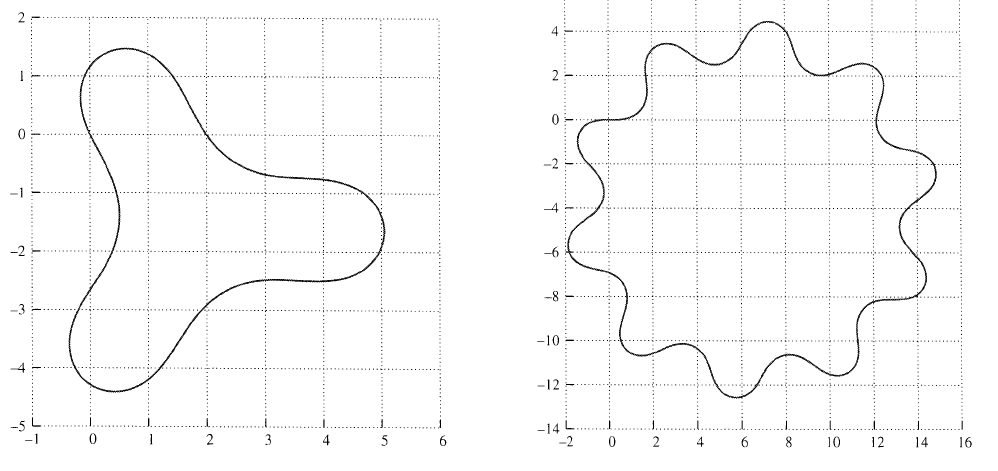
\includegraphics[scale=0.3]{pic.png}


Respectively $k(s) = \frac{1}{3} + sin(s)$ and $k(s) = \frac{1}{10} + sin(s)$.
}

\section{Conclusion}
\frame{
\frametitle{Conclusion : Remaining questions}
\begin{block}{The other cases}
What happens when the period of the curve and curvature are the same?
\end{block}
}

\end{document}
